% Provenance (never printed): see sources/outline_sources.md (Year 1: decay systems K-Ar,
% Rb-Sr, U-Pb and radiocarbon; closure temperature; dating sedimentary sequences with
% volcanic ashes; calibrating the scale). Exercise and problem values in the Book 3
% scratch calculator calc/ch25.py; figures from figdata/bachelor-1/decay_curves.py,
% isochron.py and radiocarbon.py (IntCal20, dataset bachelor-1-intcal20).
% The decay law, half-life and decay constant belong to the physics series (recalled);
% the closed system and the isochron of minerals are Book 2's (g12 age-of-the-earth),
% re-founded here with whole-rock samples and least squares. The concordia diagram and
% thermochronology are the Year 3 volume's: prose pointers only. Mass spectrometry is
% the chemistry series' (recalled). The isochron figure uses an invented rhyolite so that
% the Varden granite of the problem is not solved in the course.
\chapter{Les méthodes de datation radiométrique}\label{ch:b1:radiometric-methods}

En 2001, une équipe travaillant sur des grains détritiques de zircon des Jack Hills, en
Australie-Occidentale, en signala un qui avait cristallisé il y a
\num[uncertainty-mode=separate]{4404 \pm 8} millions d'années. Des travaux ultérieurs ont confirmé l'âge de ces
grains~: ce sont les plus anciens matériaux connus de toute sorte formés sur la Terre, et
ils montrent qu'une \omterm{def:b1:layered-earth:layers}{croûte} s'était formée moins de 160 millions d'années après la naissance du
Système solaire. À l'autre bout de l'échelle, des âges à l'argon ont placé
l'extinction de la fin du Crétacé, il y a \qty{66.00}{\Ma}, à moins de
\num{32000} ans de l'impact que l'on croit en être la cause. Les deux nombres viennent d'un comptage d'atomes~: un parent radioactif qui se désintègre à une vitesse
connue, un fils qui s'accumule. Ce chapitre explique comment de telles horloges se lisent,
pourquoi chacune date un événement différent, et comment elles accrochent la charte du
\cref{ch:b1:stratigraphic-scale} à une échelle d'années.
% ledger: wilde01:4404, uw14:jack-hills, ics:base.Paleogene, renne:kpg

\begin{omfigure}
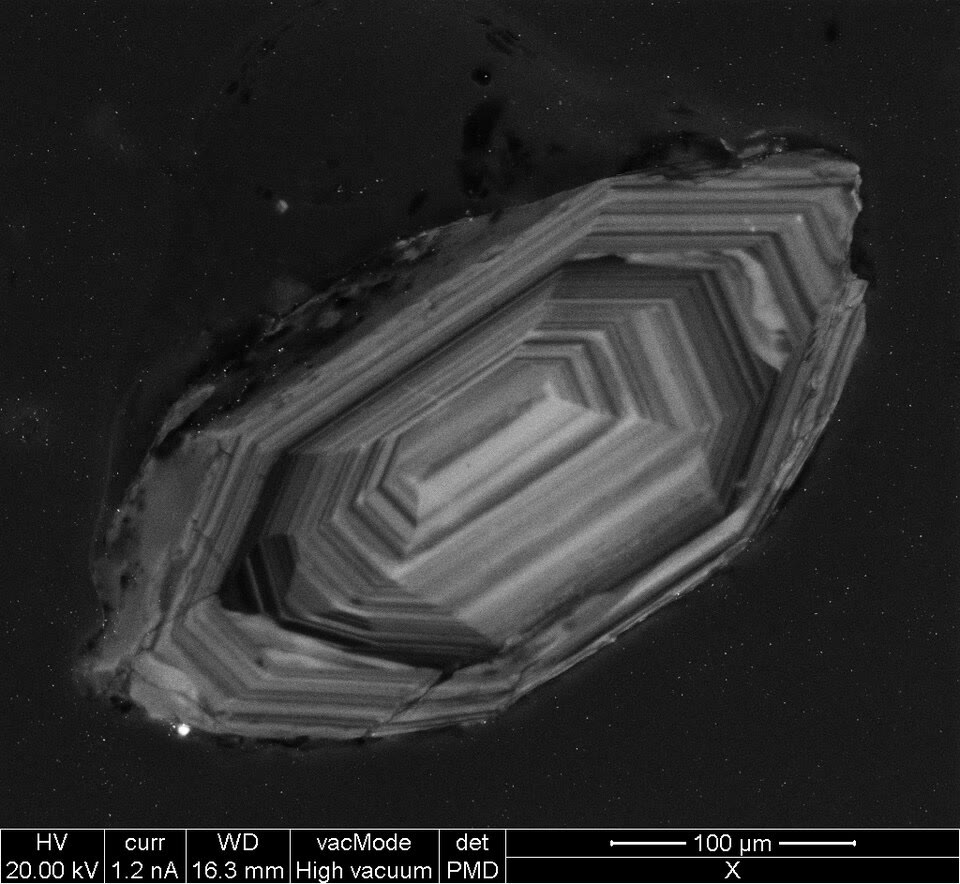
\includegraphics[width=0.5\linewidth]{images/book3/b1-zircon-cl.jpg}

{\small Un grain de zircon, long d'environ un tiers de millimètre, imagé par la
lumière qu'il émet sous le faisceau d'électrons d'un microscope électronique à balayage
(cathodoluminescence). Les bandes qui suivent les faces du cristal sont
des zones de composition légèrement différente, déposées l'une après l'autre pendant sa
croissance. Ce grain a été prélevé dans un grès, donc il est plus ancien que le grès~:
il date la roche dont il a été érodé. (Emmanuel Roquette, CC~BY-SA~4.0,
via Wikimedia Commons.)}
\label{fig:b1:radiometric-methods:zircon}
\end{omfigure}
% ledger: commons:zircon-cl

\begin{recall}
Les volumes de physique décrivent la désintégration radioactive~: les noyaux d'un isotope
radioactif se désintègrent au hasard, indépendamment de la température et de la pression, de sorte que le
nombre $N$ restant après un temps $t$ suit $N = N_0\,e^{-\lambda t}$, où
$\lambda$ est la constante de désintégration~; la demi-vie est $T = \ln 2/\lambda$. Les isotopes
d'un élément ont le même nombre de protons et des nombres de
neutrons différents~; les volumes de chimie décrivent le spectromètre de masse, qui trie les ions
selon leur masse. Au livre~2, année~12, une roche ou un \omterm{def:b1:rock-forming-minerals:mineral}{minéral} qui n'a échangé ni atomes père ni
atomes fils avec son environnement est un système fermé, et les minéraux du
granite de Varden, portés sur une \omterm{def:b1:radiometric-methods:isochron}{isochrone} rubidium--strontium, ont donné un âge de 310
millions d'années. La biotite, la muscovite et la hornblende sont les \omterm{def:b1:rock-forming-minerals:groups}{micas} et l'\omterm{def:b1:rock-forming-minerals:groups}{amphibole}
du \cref{def:b1:rock-forming-minerals:groups}. Un âge entre deux niveaux datés
peut être interpolé (\cref{prop:b1:stratigraphic-scale:interpolation}).
\end{recall}
% ledger: tulane:radiometric, villa22:rb87

\section{Les systèmes de désintégration}\label{sec:b1:radiometric-methods:systems}

Une horloge demande deux comptages~: ce qui reste du père, et la quantité de fils qu'il
a faite depuis le départ de l'horloge.

\begin{definition}[Isotope père, fils radiogénique]\label{def:b1:radiometric-methods:radiogenic}
Dans un système de désintégration utilisé pour dater, l'\emph{isotope père}\index{isotope pere@isotope père} est l'isotope radioactif dont la désintégration sert d'horloge, et le
fils est l'isotope que sa désintégration produit. Le \emph{fils
radiogénique}\index{fils radiogenique@fils radiogénique}, noté $D^*$, est la part du
fils faite par la désintégration du père dans l'échantillon depuis que l'horloge
a démarré~; le reste, $D_0$, était là depuis le début. Le nombre d'atomes du
fils mesuré aujourd'hui est $D = D_0 + D^*$.
\end{definition}

\begin{proposition}[Croissance radiogénique et équation de l'âge]\label{prop:b1:radiometric-methods:growth}
Dans un système fermé qui contient aujourd'hui $P$ atomes du père, le \omterm{def:b1:radiometric-methods:radiogenic}{fils
radiogénique} produit en un temps $t$ est
\[
  D^* = P\,\bigl(e^{\lambda t} - 1\bigr),
\]
à condition que chaque désintégration donne un atome du fils. L'âge est alors
\[
  t = \frac{1}{\lambda}\,\ln\!\left(1 + \frac{D^*}{P}\right).
\]
\end{proposition}

\begin{proof}
D'après la loi de désintégration le père comptait $P_0 = P\,e^{\lambda t}$ atomes quand l'horloge
a démarré. Dans un système fermé chaque atome père manquant est devenu un atome
fils, donc $D^* = P_0 - P = P\,(e^{\lambda t} - 1)$. Alors $e^{\lambda t} = 1 +
D^*/P$~; en prenant les logarithmes on obtient l'âge.
\end{proof}

L'âge ne dépend que d'un rapport de deux nombres d'atomes, ce que mesure le mieux un
spectromètre de masse. La figure ci-dessous montre les deux comptages en unités de
la demi-vie~: après une demi-vie $D^*/P = 1$, après deux $3$, après trois $7$
--- en général $2^n - 1$ après $n$ demi-vies.

\begin{omfigure}
\begin{tikzpicture}
\begin{axis}[omrecord, width=0.72\linewidth, height=5.6cm, xmin=0, xmax=5, ymin=0, ymax=1.05,
  xlabel={temps (demi-vies)}, ylabel={fraction du père initial},
  xtick={0,1,...,5}, ytick={0,0.25,0.5,0.75,1}]
% computed in figdata/bachelor-1/decay_curves.py (no real-world number)
\addplot[omThm, line width=1pt] table[x=n, y=P] {figdata/out/bachelor-1-decay_curves-curves.dat};
\addplot[omDef, line width=1pt] table[x=n, y=D] {figdata/out/bachelor-1-decay_curves-curves.dat};
\addplot[only marks, mark=*, mark size=1.4pt, black!60] table[x=n, y=P] {figdata/out/bachelor-1-decay_curves-marks.dat};
\addplot[only marks, mark=*, mark size=1.4pt, black!60] table[x=n, y=D] {figdata/out/bachelor-1-decay_curves-marks.dat};
\node[font=\small, text=omThm, anchor=south west] at (axis cs:0.35,0.80) {père $P$};
\node[font=\small, text=omDef, anchor=north west] at (axis cs:2.55,0.66) {fils radiogénique $D^*$};
\node[font=\scriptsize, anchor=west, inner sep=1pt] (r1) at (axis cs:0.12,0.5) {$D^*/P = 1$};
\draw[black!60, line width=0.4pt] (r1.east) -- (axis cs:0.95,0.5);
\node[font=\scriptsize, anchor=south] at (axis cs:2,0.77) {$3$};
\node[font=\scriptsize, anchor=south] at (axis cs:3,0.89) {$7$};
\node[font=\scriptsize, anchor=north] at (axis cs:4,0.915) {$15$};
\node[font=\scriptsize, anchor=north east] at (axis cs:4.97,0.95) {$31$};
\end{axis}
\end{tikzpicture}

{\small Le père et son \omterm{def:b1:radiometric-methods:radiogenic}{fils radiogénique} dans un système fermé, en fractions du
nombre initial d'atomes père, en fonction du temps compté en demi-vies. Leur somme
reste égale à un~; le rapport $D^*/P$, imprimé à chaque demi-vie entière, double
et gagne un à chaque pas.}
\label{fig:b1:radiometric-methods:decay}
\end{omfigure}

Une horloge ne se lit bien que dans une fenêtre d'âges. Bien avant une demi-vie le
fils est une minuscule fraction du père~; après de nombreuses demi-vies il reste trop peu de
père à mesurer. Le tableau ci-dessous donne les systèmes les plus utilisés, avec le matériau
auquel chacun s'applique.

\begin{table}[ht]
\centering
\small
\renewcommand{\arraystretch}{1.25}
\begin{tabular}{|l|l|c|c|>{\raggedright\arraybackslash}p{4.3cm}|}
\hline
père & fils & demi-vie (années) & $\lambda$ (par an) & matériau daté \\
\hline
$^{14}\mathrm{C}$ & $^{14}\mathrm{N}$ & \num{5700} & \num{1.216e-4} & bois, charbon de bois, os, coquilles \\
$^{40}\mathrm{K}$ & $^{40}\mathrm{Ar}$, $^{40}\mathrm{Ca}$ & \num{1.25e9} & \num{5.543e-10} & minéraux riches en potassium~: sanidine, biotite, hornblende \\
$^{87}\mathrm{Rb}$ & $^{87}\mathrm{Sr}$ & \num{4.96e10} & \num{1.3972e-11} & granites (roches totales), \omterm{def:b1:rock-forming-minerals:groups}{micas} \\
$^{147}\mathrm{Sm}$ & $^{143}\mathrm{Nd}$ & \num{1.07e11} & \num{6.46e-12} & roches et leurs minéraux (\omterm{def:b1:radiometric-methods:isochron}{isochrones}) \\
$^{235}\mathrm{U}$ & $^{207}\mathrm{Pb}$ & \num{7.04e8} & \num{9.8485e-10} & zircon \\
$^{238}\mathrm{U}$ & $^{206}\mathrm{Pb}$ & \num{4.47e9} & \num{1.55125e-10} & zircon \\
\hline
\end{tabular}
\caption{Les principaux systèmes de désintégration. Les constantes de désintégration du potassium~40 et des
deux uraniums sont les valeurs conventionnelles utilisées pour calculer les âges~; celles du
rubidium~87 et du samarium~147 sont calculées à partir des demi-vies, celle du
carbone~14 à partir de sa demi-vie de \num{5700} ans.}
\label{tab:b1:radiometric-methods:systems}
\end{table}
% ledger: iaea:c14, iaea:k40-branches, amherst:constants, villa22:rb87, iaea:sm147, iaea:isotopes, tulane:kar, tulane:upb-zircon, tulane:c14

Deux jeux de nombres sont en usage pour les mêmes noyaux, et un âge doit dire lequel
il a employé. Les tables de données nucléaires donnent au potassium~40 une demi-vie de
\num{1.248e9} ans et envoient \qty{10.72}{\percent} de ses désintégrations vers l'argon~; les
constantes conventionnellement utilisées en géochronologie donnent $\lambda = \num{5.543e-10}$ par an (une demi-vie de \num{1.2505e9}
ans) et envoient $0.581/5.543 = \qty{10.48}{\percent}$ des désintégrations vers l'argon.
Les âges au radiocarbone, comme l'explique la \cref{sec:b1:radiometric-methods:kar}, sont
calculés avec une demi-vie de \num{5568} ans que l'on sait trop courte. Les
écarts atteignent quelques pour cent, bien plus que les \qty{0.01}{\percent} auxquels
les meilleurs âges sont désormais donnés (\cref{sec:b1:radiometric-methods:sediments}).
L'incertitude sur les constantes de désintégration du potassium~40 lui-même, un noyau à
deux branches et à longue demi-vie, limite l'exactitude de ses âges.
% ledger: iaea:k40-branches, amherst:constants, sp77:conventional-age, ics:base.Triassic, nmgrl:arar

\begin{proposition}[Précision d'un âge]\label{prop:b1:radiometric-methods:precision}
Si le rapport $R = D^*/P$ est mesuré avec l'incertitude-type $\sigma_R$,
l'âge porte l'incertitude
\[
  \sigma_t = \frac{\sigma_R}{\lambda\,(1 + R)}.
\]
\end{proposition}

\begin{proof}
Pour une petite erreur $\delta R$, l'âge $t = \ln(1+R)/\lambda$ varie de
$\delta t = t'(R)\,\delta R = \delta R/\bigl(\lambda(1 + R)\bigr)$.
\end{proof}

Pour un échantillon jeune, $R$ est petit et $\sigma_t \approx \sigma_R/\lambda$~: l'erreur
absolue sur l'âge est fixée par la qualité de mesure d'une petite quantité de fils. Une
longue demi-vie (petit $\lambda$) l'amplifie. C'est pourquoi
rubidium--strontium et uranium--plomb servent pour les roches de plus d'environ dix
millions d'années, tandis que potassium--argon atteint des roches aussi jeunes qu'environ dix
mille ans, et que le radiocarbone couvre les \num{70000} dernières années.
% ledger: tulane:ranges

\section{Les isochrones}\label{sec:b1:radiometric-methods:isochrons}

L'équation de l'âge exige $D^*$, mais l'instrument mesure $D = D_0 + D^*$, et
$D_0$ est rarement nul~: le strontium~87 est présent dans chaque \omterm{def:b1:rock-forming-minerals:mineral}{minéral} qui a pris du
strontium en se formant. L'\omterm{def:b1:radiometric-methods:isochron}{isochrone} élimine $D_0$ en mesurant plusieurs
échantillons qui sont partis de la même composition isotopique de l'élément fils.

\begin{definition}[Isochrone, rapport initial]\label{def:b1:radiometric-methods:isochron}
Soit $S$ un isotope stable de l'élément fils qu'aucune désintégration ne produit
($^{86}\mathrm{Sr}$ pour le strontium, $^{144}\mathrm{Nd}$ pour le néodyme). Une
\emph{isochrone}\index{isochrone} est la droite sur laquelle se placent, dans un graphe
de $y = D/S$ en fonction de $x = P/S$, des échantillons formés en même temps avec la
même valeur de $D/S$ et restés des systèmes fermés depuis. Cette valeur de départ commune
$y_0 = (D/S)_0$ est le \emph{rapport initial}\index{rapport initial}.
\end{definition}
% ledger: tulane:radiometric, tulane:c14

\begin{theorem}[L'isochrone]\label{thm:b1:radiometric-methods:isochron}
Des échantillons formés en même temps avec le même \omterm{def:b1:radiometric-methods:isochron}{rapport initial} $y_0$, et restés
des systèmes fermés pendant un temps $t$, vérifient
\[
  y = y_0 + \bigl(e^{\lambda t} - 1\bigr)\,x .
\]
Leurs points se placent sur une droite de pente $m = e^{\lambda t} - 1$ et
d'ordonnée à l'origine $y_0$, et $t = \ln(1+m)/\lambda$.
\end{theorem}

\begin{proof}
Pour chaque échantillon, $D = D_0 + P\,(e^{\lambda t} - 1)$ d'après la
\cref{prop:b1:radiometric-methods:growth}. Le nombre d'atomes de $S$ n'a pas
changé, puisque $S$ est stable, produit par aucune désintégration, et que le système est fermé~;
en divisant par lui on obtient $y = y_0 + (e^{\lambda t} - 1)\,x$, avec $y_0$ le même pour
tous les échantillons par hypothèse.
\end{proof}

Quand un granite a cristallisé, tous ses échantillons avaient le même $y_0$ et se plaçaient sur une
droite horizontale~; chacun est depuis monté en proportion de son $x$, et la droite
a tourné autour de son ordonnée à l'origine. Les échantillons ont besoin de valeurs de $x$ différentes pour
bien définir la pente~: des minéraux riches et pauvres en rubidium, comme au livre~2,
ou des échantillons de roche totale pris dans des parties plus ou moins évoluées d'une même intrusion. Un
point hors de la droite marque un échantillon qui n'était pas fermé, ou qui ne partageait pas
le \omterm{def:b1:radiometric-methods:isochron}{rapport initial}. Le \omterm{def:b1:radiometric-methods:isochron}{rapport initial} est lui-même un traceur~: un magma issu du \omterm{def:b1:layered-earth:layers}{manteau}
hérite d'un faible $^{87}\mathrm{Sr}/^{86}\mathrm{Sr}$, environ $0.7025$, et un magma issu de
\omterm{def:b1:layered-earth:layers}{croûte} continentale fondue d'un rapport élevé, environ $0.710$, parce que la \omterm{def:b1:layered-earth:layers}{croûte} est riche en
rubidium et a fait davantage de strontium~87 au cours des âges.
% ledger: tulane:radiometric, tulane:sr-initial

Les points réels ne tombent jamais exactement sur une droite. L'estimation usuelle de la droite est
celle qui rend aussi petits que possible les carrés des distances verticales des points à elle.

\begin{proposition}[La droite des moindres carrés]\label{prop:b1:radiometric-methods:lsq}
Soit $(x_i, y_i)$, $i = 1, \dots, n$, des points avec au moins deux $x_i$ différents,
de moyennes $\bar x$ et $\bar y$, et soit
\[
  S_{xx} = \sum_i (x_i - \bar x)^2, \qquad S_{xy} = \sum_i (x_i - \bar x)(y_i - \bar y).
\]
La droite $y = b + m x$ qui minimise $Q(b, m) = \sum_i (y_i - b - m x_i)^2$ a pour coefficients
\[
  m = \frac{S_{xy}}{S_{xx}}, \qquad b = \bar y - m\,\bar x ,
\]
et passe par le centre de gravité $(\bar x, \bar y)$.
\end{proposition}

\begin{proof}
$Q$ est une somme de carrés, un polynôme de degré deux en $(b, m)$ qui tend vers
l'infini dans toutes les directions, donc il atteint son minimum là où les deux dérivées
partielles s'annulent. $\partial Q/\partial b = -2 \sum_i (y_i - b - m x_i) = 0$
donne $n\bar y = n b + n m \bar x$, donc $b = \bar y - m \bar x$~: la droite passe
par le centre de gravité. En substituant, $y_i - b - m x_i = (y_i - \bar y) - m(x_i -
\bar x)$, et $\partial Q/\partial m = -2 \sum_i x_i \bigl[(y_i - \bar y) - m(x_i
- \bar x)\bigr] = 0$. Comme $\sum_i (y_i - \bar y) = \sum_i (x_i - \bar x) = 0$, on peut
remplacer $x_i$ par $x_i - \bar x$ dans cette somme, ce qui donne $S_{xy} - m S_{xx} = 0$.
$S_{xx} > 0$ parce que les $x_i$ ne sont pas tous égaux.
\end{proof}

La dispersion des points autour de la droite donne l'incertitude de la pente.
Avec les résidus $r_i = y_i - b - m x_i$, l'écart-type de la
dispersion est $s = \sqrt{\sum_i r_i^2/(n-2)}$ --- deux degrés de liberté sont utilisés
par les deux paramètres --- et les incertitudes-types de la pente et de
l'ordonnée à l'origine sont
\[
  \sigma_m = \frac{s}{\sqrt{S_{xx}}}, \qquad
  \sigma_b = s\,\sqrt{\frac1n + \frac{\bar x^2}{S_{xx}}} .
\]
Ces deux résultats de statistique sont admis ici~; l'âge porte alors
$\sigma_t = \sigma_m/\bigl(\lambda(1 + m)\bigr)$, par l'argument de la
\cref{prop:b1:radiometric-methods:precision}. Ils montrent ce qui fait une bonne
\omterm{def:b1:radiometric-methods:isochron}{isochrone}~: beaucoup de points, largement répartis en $x$ (un grand $S_{xx}$), avec peu de
dispersion.

\begin{method}[Ajuster une isochrone]\label{met:b1:radiometric-methods:isochron}
\begin{enumerate}
  \item Mesurer $x = P/S$ et $y = D/S$ sur au moins quatre échantillons d'un même corps,
        choisis pour répartir $x$ le plus largement possible.
  \item Les porter~; mettre de côté, en justifiant, tout point nettement hors de la tendance.
  \item Calculer $\bar x$, $\bar y$, $S_{xx}$, $S_{xy}$, puis $m = S_{xy}/S_{xx}$
        et $b = \bar y - m \bar x$.
  \item Calculer les résidus, $s$, $\sigma_m$ et $\sigma_b$.
  \item L'âge est $t = \ln(1+m)/\lambda$, avec $\sigma_t =
        \sigma_m/\bigl(\lambda(1+m)\bigr)$~; le \omterm{def:b1:radiometric-methods:isochron}{rapport initial} est $b \pm \sigma_b$.
\end{enumerate}
\end{method}

\begin{example}[Une rhyolite inventée]\label{ex:b1:radiometric-methods:rhyolite}
Six échantillons de roche totale d'une série de laves rhyolitiques (données d'exercice) donnent~:
\begin{center}
\small
\begin{tabular}{|l|cccccc|}
\hline
$x = {}^{87}\mathrm{Rb}/^{86}\mathrm{Sr}$ & 1.85 & 4.62 & 9.30 & 14.75 & 21.20 & 27.60 \\
$y = {}^{87}\mathrm{Sr}/^{86}\mathrm{Sr}$ & 0.71732 & 0.73332 & 0.76164 & 0.79420 & 0.83226 & 0.87028 \\
\hline
\end{tabular}
\end{center}
Ici $\bar x = 13.22$, $\bar y = 0.784837$, $S_{xx} = 491.41$ et
$S_{xy} = 2.92308$, donc $m = 0.0059484$ et $b = 0.70620$. Les résidus donnent
$s = 0.00024$, $\sigma_m = \num{1.10e-5}$ et $\sigma_b = 0.00018$. L'âge est
$t = \ln(1.0059484)/\num{1.3972e-11} = \qty{424.5}{\Ma}$, avec
$\sigma_t = \num{1.10e-5}/(\num{1.3972e-11} \times 1.0059) = \qty{0.8}{\Ma}$~:
\qty[uncertainty-mode=separate]{424.5(8)}{\Ma}, \omterm{def:b1:radiometric-methods:isochron}{rapport initial}
\num[uncertainty-mode=separate]{0.70620(18)} (figure ci-dessous).
\end{example}
% values: isochron.py (slope 0.005948361, intercept 0.7061993, age 424.4732, sigma 0.7827871); ledger: villa22:rb87

\begin{omfigure}
\begin{tikzpicture}
\begin{axis}[omrecord, width=0.74\linewidth, height=6cm, xmin=0, xmax=30, ymin=0.70, ymax=0.88,
  xlabel={$^{87}\mathrm{Rb}/^{86}\mathrm{Sr}$}, ylabel={$^{87}\mathrm{Sr}/^{86}\mathrm{Sr}$},
  ytick={0.70,0.72,...,0.88},
  y tick label style={/pgf/number format/.cd, fixed, fixed zerofill, precision=2}]
% computed in figdata/bachelor-1/isochron.py (exercise data, invented rhyolite); ledger: villa22:rb87
\addplot[black!60, densely dotted, line width=0.7pt] table[x=x, y=y] {figdata/out/bachelor-1-isochron-initial.dat};
\addplot[omDef, line width=0.9pt] table[x=x, y=y] {figdata/out/bachelor-1-isochron-line.dat};
\addplot[omThm, only marks, mark=*, mark size=2pt] table[x=x, y=y] {figdata/out/bachelor-1-isochron-points.dat};
\node[font=\scriptsize, text=omDef, anchor=south east, align=right] at (axis cs:19,0.83)
  {pente des moindres carrés $0.005948$\\ âge \qty[uncertainty-mode=separate]{424.5(8)}{\Ma}};
\node[font=\scriptsize, text=black!70, anchor=south west] at (axis cs:9,0.7068)
  {rapport initial $0.70620$, à la formation des laves};
\end{axis}
\end{tikzpicture}

{\small Une \omterm{def:b1:radiometric-methods:isochron}{isochrone} rubidium--strontium de six échantillons de roche totale d'une
rhyolite inventée (données d'exercice). Les points se dispersent légèrement autour de la droite
des moindres carrés, qui passe par leur centre de gravité~; la droite en pointillés est la place où tous
se trouvaient à la formation des laves.}
\label{fig:b1:radiometric-methods:isochron}
\end{omfigure}

\begin{inthelab}[Peser des isotopes]
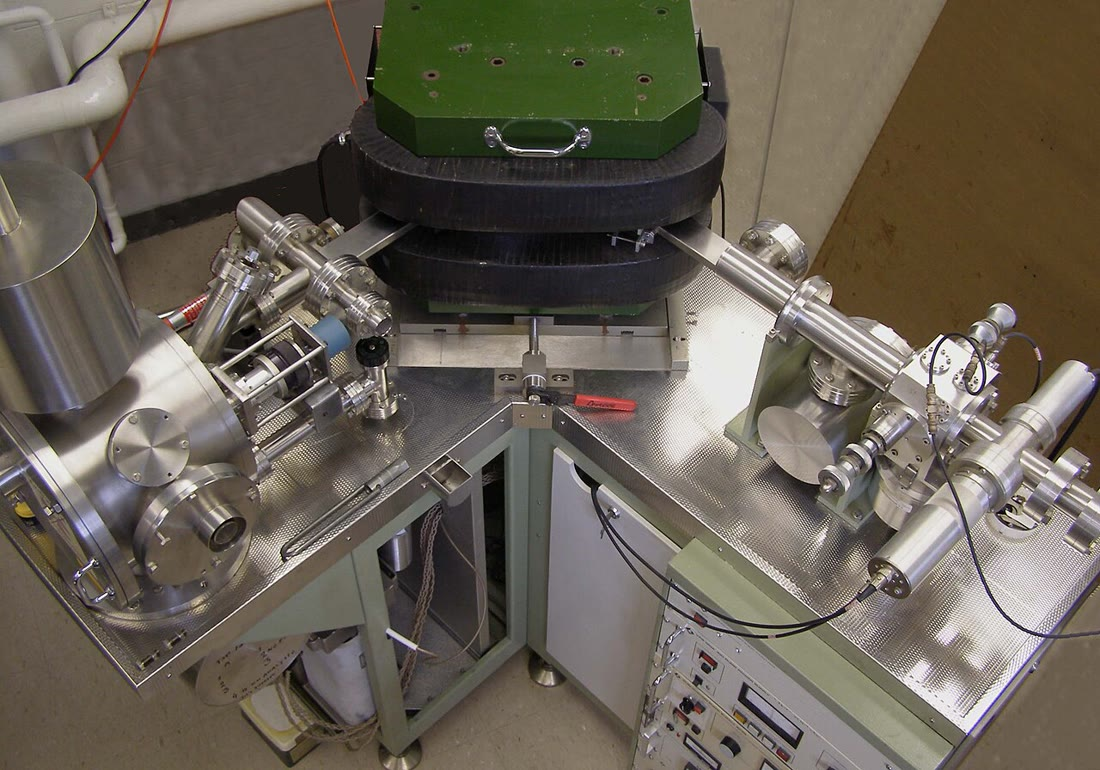
\includegraphics[width=0.42\linewidth]{images/book3/b1-tims.jpg}\hfill
\begin{minipage}[b]{0.55\linewidth}
Un spectromètre de masse à ionisation thermique (à gauche) mesure les rapports isotopiques
d'éléments tels que le strontium. L'élément, séparé de l'échantillon dissous par
la chimie, est déposé sur un filament métallique sous vide~; chauffé, il émet des ions,
qui sont accélérés et courbés par le champ du grand électroaimant (les
bobines noires au centre), les ions légers plus que les lourds, si bien que chaque
isotope atteint son propre collecteur. Les rapports d'isotopes sont ce que l'instrument
mesure le mieux, c'est pourquoi les méthodes fondées sur les seuls rapports sont les plus précises.
(Photographie~: Radiogenic, CC0, via Wikimedia Commons.)
\end{minipage}
\end{inthelab}
% ledger: commons:tims, amherst:constants

\section{Potassium--argon, uranium--plomb et radiocarbone}\label{sec:b1:radiometric-methods:kar}

\subsection*{Un père à deux fils}

\begin{definition}[Désintégration à embranchement]\label{def:b1:radiometric-methods:branching}
Un père subit une \emph{désintégration à embranchement}\index{desintegration a embranchement@désintégration à embranchement} quand ses noyaux
se désintègrent par deux voies ou plus vers des fils différents. Chaque voie $i$ a sa propre
constante de désintégration partielle $\lambda_i$~; le père se désintègre avec la constante totale
$\lambda = \sum_i \lambda_i$, et une fraction $\lambda_i/\lambda$ des désintégrations
emprunte la voie~$i$. Le potassium~40 se désintègre en calcium~40 avec $\lambda_\beta =
\num{4.962e-10}$ par an et en argon~40 avec $\lambda_e = \num{0.581e-10}$ par
an.
\end{definition}
% ledger: amherst:constants, iaea:k40-branches

\begin{proposition}[L'âge potassium--argon]\label{prop:b1:radiometric-methods:kar}
Un \omterm{def:b1:rock-forming-minerals:mineral}{minéral} qui a gardé tout l'argon qui s'est formé en lui, et n'en contenait aucun à sa
formation, contient après un temps $t$
\[
  {}^{40}\mathrm{Ar}^* = \frac{\lambda_e}{\lambda}\;{}^{40}\mathrm{K}\,\bigl(e^{\lambda t} - 1\bigr),
  \qquad\text{donc}\qquad
  t = \frac{1}{\lambda}\,\ln\!\left(1 + \frac{\lambda}{\lambda_e}\,
      \frac{{}^{40}\mathrm{Ar}^*}{{}^{40}\mathrm{K}}\right),
\]
où ${}^{40}\mathrm{K}$ est le nombre d'atomes de potassium~40 aujourd'hui et $\lambda =
\lambda_\beta + \lambda_e$.
\end{proposition}

\begin{proof}
Le père se désintègre avec la constante totale $\lambda$, quelle que soit la voie, donc d'après la
\cref{prop:b1:radiometric-methods:growth} le nombre de désintégrations pendant le temps $t$ est
${}^{40}\mathrm{K}\,(e^{\lambda t} - 1)$. Chaque désintégration prend la voie de l'argon avec la
probabilité $\lambda_e/\lambda$, indépendamment des autres~; sur le très
grand nombre de désintégrations, la fraction qui a donné de l'argon est $\lambda_e/\lambda$. Cela
donne ${}^{40}\mathrm{Ar}^*$~; la résolution en $t$ donne l'âge.
\end{proof}

L'exposant contient la constante totale et le facteur devant la constante partielle~:
employer $\lambda_e$ dans l'exposant, comme si l'argon était la seule voie, donnerait
un âge extrêmement faux. La branche du calcium porte les neuf dixièmes des désintégrations mais est
inutile pour la datation, parce que le calcium~40 est l'isotope courant d'un élément
abondant dans les roches~; l'argon, gaz noble, s'échappe d'un liquide magmatique, si bien qu'un cristal
démarre avec presque aucun. Le potassium~40 fait \qty{0.0117}{\percent} des atomes de
potassium. La méthode exige les quantités absolues de potassium et d'argon,
mesurées séparément. L'argon de l'air, présent dans toute roche, est reconnu par
son argon~36 et soustrait avec le rapport atmosphérique
$^{40}\mathrm{Ar}/^{36}\mathrm{Ar} = 295.5$.
% ledger: tulane:kar, iaea:k40-branches, amherst:constants, nmgrl:kar

La méthode échoue de deux façons. L'argon en excès donne des âges trop vieux~: une lave qui
refroidit vite peut piéger de l'argon du \omterm{def:b1:layered-earth:layers}{manteau} dans des bulles, et les laves historiques
donnent en général des âges potassium--argon de 1 à 2 millions d'années, une erreur qui
ne compte que pour les roches jeunes. La perte d'argon les rend trop jeunes~: la plupart des minéraux
perdent de l'argon quand on les chauffe au-dessus d'environ \qty{300}{\celsius}, si bien qu'un
métamorphisme ultérieur remet l'horloge à zéro en tout ou partie, et une perte partielle donne un âge
entre les deux événements qui ne date ni l'un ni l'autre. On préfère les minéraux riches en potassium~:
sanidine et biotite, puis \omterm{def:b1:rock-forming-minerals:groups}{plagioclase} ou hornblende.
% ledger: tulane:kar, nmgrl:kar

La méthode argon--argon ne mesure que des rapports. L'échantillon est irradié par des
neutrons rapides au cœur d'un réacteur nucléaire, à côté d'un \omterm{def:b1:rock-forming-minerals:mineral}{minéral} étalon
d'âge connu~; la réaction transforme une partie de son potassium~39 en argon~39, qui
tient alors lieu de potassium, et l'étalon donne le rendement de la réaction. Les
deux isotopes sont mesurés ensemble dans le même gaz. L'échantillon peut alors être
chauffé par paliers, avec un four ou un laser~; chaque palier donne un âge, et les
âges sont portés en fonction de la fraction cumulée d'argon~39 libérée, un spectre
d'âge. Les paliers qui s'accordent dans leurs erreurs forment un plateau~; un spectre
sans plateau avertit que le \omterm{def:b1:rock-forming-minerals:mineral}{minéral} n'est pas resté fermé. Le synchronisme de
l'impact et de l'extinction de la fin du Crétacé repose sur des âges argon--argon.
% ledger: amherst:arar, nmgrl:arar, renne:kpg

\subsection*{Deux horloges à uranium}

L'uranium a deux isotopes de longue vie, l'uranium~238 se désintégrant en plomb~206
et l'uranium~235 en plomb~207, à des vitesses différentes~; aujourd'hui
$^{235}\mathrm{U}/^{238}\mathrm{U} = 0.0072567$, un atome sur 137.8. Un \omterm{def:b1:rock-forming-minerals:mineral}{minéral}
contenant de l'uranium porte donc deux horloges indépendantes, chacune avec sa propre
équation de croissance, ${}^{206}\mathrm{Pb}^* = {}^{238}\mathrm{U}\,(e^{\lambda_{238} t} - 1)$
et ${}^{207}\mathrm{Pb}^* = {}^{235}\mathrm{U}\,(e^{\lambda_{235} t} - 1)$. Si les
deux âges s'accordent, on dit qu'ils sont concordants, et l'accord est un test
de la fermeture du \omterm{def:b1:rock-forming-minerals:mineral}{minéral}, que nulle horloge seule ne peut fournir. Le désaccord
vient surtout de plomb perdu par des parties du cristal endommagées par le rayonnement
de l'uranium lui-même~; un graphe des deux rapports l'un en fonction de l'autre, le
diagramme concordia, retrouve alors à la fois l'âge du cristal et celui de
l'événement qui lui a fait perdre du plomb --- un outil du volume de troisième année.
% ledger: amherst:constants, tulane:upb-zircon

Le zircon, $\mathrm{ZrSiO_4}$, est le \omterm{def:b1:rock-forming-minerals:mineral}{minéral} de choix~: il admet l'uranium dans sa
structure mais presque pas de plomb, si bien que presque tout son plomb est radiogénique~; il est
dur, résiste à l'altération et survit au métamorphisme, si bien que les grains érodés
d'une roche gardent son âge dans les sables qui en dérivent. L'apatite et le sphène sont employés
aussi, moins souvent.
% ledger: tulane:upb-zircon, commons:zircon-cl

\subsection*{Le radiocarbone}

Le carbone~14 est fabriqué en continu dans la haute atmosphère à partir de l'azote~14 frappé
par les rayons cosmiques. Il rejoint le carbone de l'atmosphère~; les organismes vivants
échangent du carbone avec l'atmosphère et gardent sa proportion de carbone~14. À
la mort l'échange cesse et le carbone~14 se désintègre en azote~14. Puisque la
proportion initiale est celle de l'atmosphère, l'âge découle de la loi de désintégration
seule, sans \omterm{def:b1:radiometric-methods:isochron}{isochrone}~: $t = -\tau \ln(A/A_0)$, où $A$ est
l'activité du carbone de l'échantillon, $A_0$ celle du carbone vivant et $\tau =
1/\lambda$ la vie moyenne. Le bois, le charbon de bois, les os, les dents et les coquilles se datent ainsi,
jusqu'à quelques dizaines de milliers d'années~: environ \num{70000} ans au plus.
% ledger: tulane:c14, iaea:c14

\begin{definition}[Âge radiocarbone, courbe d'étalonnage]\label{def:b1:radiometric-methods:radiocarbon}
L'\emph{âge radiocarbone}\index{age radiocarbone@âge radiocarbone} (conventionnel) d'un échantillon est
\[
  t = -8033 \,\ln \frac{A_{\mathrm{SN}}}{A_{\mathrm{ON}}} \ \text{ans BP},
\]
où $A_{\mathrm{SN}}$ est l'activité du carbone de l'échantillon et
$A_{\mathrm{ON}}$ celle de l'étalon de référence~; il utilise la demi-vie de
\num{5568} ans (vie moyenne \num{8033} ans), normalise les activités pour
le fractionnement isotopique du carbone ($\delta^{13}\mathrm{C} = \qty{-25}{\permil}$),
et compte les années avant 1950 apr.~J.-C. (BP, «~before present~», avant le présent). Une
\emph{courbe d'étalonnage}\index{courbe d'etalonnage@courbe d'étalonnage} donne l'âge radiocarbone
d'échantillons d'âge calendaire connu~; lue à l'envers, elle convertit un âge radiocarbone en
un intervalle d'âges calendaires (cal BP).
\end{definition}
% ledger: sp77:conventional-age, reimer20:intcal20

L'\omterm{def:b1:radiometric-methods:radiocarbon}{âge radiocarbone} n'est pas un âge en années calendaires, pour deux raisons. La
demi-vie de \num{5568} ans, valeur de Libby, conservée par convention, est plus courte que la vraie valeur de \num{5700} ans, si bien que les \omterm{def:b1:radiometric-methods:radiocarbon}{âges radiocarbone} sont
environ \qty{2.4}{\percent} trop courts. Plus important, la proportion de carbone~14 dans
l'atmosphère n'a pas été constante. La \omterm{def:b1:radiometric-methods:radiocarbon}{courbe d'étalonnage} mesure les deux effets
ensemble, sur des archives datées indépendamment~: cernes d'arbres jusqu'à environ
\num{13900} cal BP, et au-delà des séquences flottantes de cernes, des sédiments lacustres et
marins, des dépôts de grottes et des coraux, jusqu'à \num{55000} cal BP (figure ci-dessous).
% ledger: sp77:conventional-age, iaea:c14, reimer20:intcal20

\begin{omfigure}
\begin{tikzpicture}
\begin{axis}[name=main, omrecord, width=0.5\linewidth, height=6cm, xmin=0, xmax=12, ymin=0, ymax=12,
  xlabel={âge calendaire (milliers de cal BP)}, ylabel={âge radiocarbone (milliers de BP)},
  xtick={0,2,...,12}, ytick={0,2,...,12}]
% figdata/bachelor-1/radiocarbon.py, IntCal20 (dataset bachelor-1-intcal20); ledger: data:b3-intcal20
\addplot[black!50, dashed, domain=0:12, samples=2] {x};
\addplot[omDef, line width=0.9pt] table[x=cal, y=c14] {figdata/out/bachelor-1-radiocarbon-curve.dat};
\draw[omThm, line width=0.6pt] (axis cs:2.3,2.3) rectangle (axis cs:2.9,2.9);
\node[font=\scriptsize, anchor=east, text=black!60] at (axis cs:8.4,10.4) {âges égaux};
\node[font=\scriptsize, text=omDef, anchor=north west] at (axis cs:7.4,5.6) {IntCal20};
\end{axis}
\begin{axis}[at={(main.east)}, anchor=west, xshift=2.1cm, omrecord, width=0.38\linewidth, height=6cm,
  xmin=2300, xmax=2900, ymin=2300, ymax=2900, xlabel={âge calendaire (cal BP)}, ylabel={âge radiocarbone (BP)},
  xtick={2300,2500,2700,2900}, ytick={2300,2500,2700,2900},
  x tick label style={/pgf/number format/.cd, set thousands separator={}},
  y tick label style={/pgf/number format/.cd, set thousands separator={}}]
\addplot[name path=hi, draw=none, forget plot] table[x=cal, y=hi] {figdata/out/bachelor-1-radiocarbon-zoom.dat};
\addplot[name path=lo, draw=none, forget plot] table[x=cal, y=lo] {figdata/out/bachelor-1-radiocarbon-zoom.dat};
\addplot[omDef!25, forget plot] fill between[of=hi and lo];
\addplot[omDef, line width=0.8pt] table[x=cal, y=c14] {figdata/out/bachelor-1-radiocarbon-zoom.dat};
\addplot[omThm, line width=0.6pt, domain=2300:2900, samples=2] {2480};
\draw[omThm, densely dotted] (axis cs:2495,2300) -- (axis cs:2495,2480);
\draw[omThm, densely dotted] (axis cs:2699,2300) -- (axis cs:2699,2480);
\node[font=\scriptsize, text=omThm, anchor=south west] at (axis cs:2310,2485) {$2480$ BP};
\end{axis}
\end{tikzpicture}

{\small À gauche~: la \omterm{def:b1:radiometric-methods:radiocarbon}{courbe d'étalonnage} IntCal20 sur les \num{12000} dernières années,
\omterm{def:b1:radiometric-methods:radiocarbon}{âge radiocarbone} en fonction de l'âge calendaire~; la ligne en tirets est la place où les deux seraient
égaux. À droite~: l'encadré de gauche agrandi, avec la bande d'une incertitude-type
de la courbe. Entre \num{2500} et \num{2700} cal BP la courbe
est presque plate~: un \omterm{def:b1:radiometric-methods:radiocarbon}{âge radiocarbone} de 2480 ans BP correspond à des âges calendaires
d'environ \num{2495} à \num{2699} cal BP.}
\label{fig:b1:radiometric-methods:intcal}
\end{omfigure}
% ledger: data:b3-intcal20, reimer20:intcal20

À \num{2000} cal BP la courbe donne \num[uncertainty-mode=separate]{2070 \pm 14} ans BP~; à
\num{12000} cal BP, \num{10306}~: les \omterm{def:b1:radiometric-methods:radiocarbon}{âges radiocarbone} y sont plus jeunes de \num{1694} ans
que les âges calendaires, bien plus que les \qty{2.4}{\percent} de la
demi-vie. La courbe ondule, et là où elle est plate un \omterm{def:b1:radiometric-methods:radiocarbon}{âge radiocarbone} correspond à un
long intervalle d'âges calendaires, si précise que soit la mesure.
% ledger: data:b3-intcal20

\begin{dated}{2020}
% ledger: reimer20:intcal20
La courbe en usage pour l'hémisphère Nord est IntCal20, publiée en 2020. Elle a
remplacé IntCal13, en ajoutant de nouvelles données et en prolongeant la courbe jusqu'à \num{55000} cal BP,
avec des courbes distinctes pour l'hémisphère Sud et pour l'océan de surface.
Les \omterm{def:b1:radiometric-methods:radiocarbon}{courbes d'étalonnage} sont révisées à mesure que de nouvelles archives sont mesurées, si bien qu'un âge
calendaire doit nommer la courbe qui l'a produit.
\end{dated}

\section{La température de fermeture}\label{sec:b1:radiometric-methods:closure}

Un \omterm{def:b1:rock-forming-minerals:mineral}{minéral} qui cristallise à partir d'un magma à \qty{800}{\celsius} ne met pas son horloge
en marche tout de suite. Tant qu'il est chaud, des atomes du fils --- l'argon surtout ---
diffusent à travers son réseau et s'échappent~; ce n'est que lorsqu'il s'est assez refroidi que
la diffusion devient trop lente pour compter, et que le fils commence à s'accumuler.
% ledger: leeds:closure, tulane:kar, tulane:magma-types

\begin{definition}[Température de fermeture, âge de refroidissement]\label{def:b1:radiometric-methods:closure}
La \emph{température de fermeture}\index{temperature de fermeture@température de fermeture} d'un \omterm{def:b1:rock-forming-minerals:mineral}{minéral} pour un
système de désintégration est la température en dessous de laquelle les atomes père et fils ne
diffusent plus dans son réseau, ni vers l'intérieur ni vers l'extérieur, assez vite pour compter, si bien que le
\omterm{def:b1:rock-forming-minerals:mineral}{minéral} se comporte comme un système fermé. Un \emph{âge de refroidissement}\index{age de refroidissement@âge de refroidissement} est un
âge mesuré dans un \omterm{def:b1:rock-forming-minerals:mineral}{minéral} formé au-dessus de sa température de fermeture~: il date
le moment où le \omterm{def:b1:rock-forming-minerals:mineral}{minéral} s'est refroidi en passant par cette température, non le moment où il
s'est formé.
\end{definition}
% ledger: leeds:closure

Les \omterm{def:b1:radiometric-methods:closure}{températures de fermeture} diffèrent selon le \omterm{def:b1:rock-forming-minerals:mineral}{minéral}, parce que les réseaux diffèrent, et selon
l'élément, parce que des atomes différents diffusent à travers un même réseau à des vitesses différentes
(figure ci-dessous). Elles sont approximatives~: deux tables donnent \qty{280}{\celsius} et
\qty{350}{\celsius} pour l'argon dans la biotite, \qty{530}{\celsius} et
\qty{550}{\celsius} pour l'argon dans la hornblende. Les traces de fission, sillons de dégâts
laissés dans un cristal par la fission spontanée de noyaux d'uranium, guérissent à des
températures plus basses encore.
% ledger: leeds:closure, amherst:closure

\begin{omfigure}
\begin{tikzpicture}
\begin{axis}[width=0.8\linewidth, height=7cm, xbar, bar width=7pt, xmin=0, xmax=850,
  xlabel={température de fermeture (\unit{\celsius})},
  symbolic y coords={zrupb,spupb,hbar,mssr,msar,btsr,btar,zrft,kfsar,apft},
  ytick={zrupb,spupb,hbar,mssr,msar,btsr,btar,zrft,kfsar,apft}, y dir=reverse, enlarge y limits=0.07,
  yticklabels={{zircon, U--Pb},{sphène, U--Pb},{hornblende, K--Ar},{muscovite, Rb--Sr},{muscovite, K--Ar},{biotite, Rb--Sr},{biotite, K--Ar},{zircon, traces de fission},{feldspath potassique, K--Ar},{apatite, traces de fission}},
  y tick label style={font=\scriptsize}, x tick label style={font=\scriptsize},
  axis x line*=bottom, axis y line*=left]
% ledger: leeds:closure (values as tabulated; > lower bound, ~ approximate, ranges and +- as given)
\addplot[fill=omDef!55, draw=omDef, error bars/.cd, x dir=both, x explicit]
  coordinates {(750,zrupb) (650,spupb) (530,hbar) +- (40,0) (500,mssr) (350,msar) (320,btsr)
               (280,btar) +- (40,0) (200,zrft) +- (25,0) (130,kfsar) (105,apft) +- (10,0)};
\node[font=\scriptsize, anchor=west] at (axis cs:755,zrupb) {$> 750$};
\node[font=\scriptsize, anchor=west] at (axis cs:655,spupb) {$> 650$};
\node[font=\scriptsize, anchor=west] at (axis cs:575,hbar) {$530 \pm 40$};
\node[font=\scriptsize, anchor=west] at (axis cs:505,mssr) {$500$};
\node[font=\scriptsize, anchor=west] at (axis cs:355,msar) {$\approx 350$};
\node[font=\scriptsize, anchor=west] at (axis cs:325,btsr) {$320$};
\node[font=\scriptsize, anchor=west] at (axis cs:325,btar) {$280 \pm 40$};
\node[font=\scriptsize, anchor=west] at (axis cs:230,zrft) {$175$--$225$};
\node[font=\scriptsize, anchor=west] at (axis cs:135,kfsar) {$\approx 130$, avec fuites};
\node[font=\scriptsize, anchor=west] at (axis cs:120,apft) {$105 \pm 10$};
\end{axis}
\end{tikzpicture}

{\small \omterm{def:b1:radiometric-methods:closure}{Températures de fermeture} des principales horloges \omterm{def:b1:rock-forming-minerals:mineral}{minérales}, d'après une table publiée.
U--Pb est uranium--plomb, K--Ar potassium--argon (et argon--argon), Rb--Sr
rubidium--strontium. Pour les traces de fission, la valeur est la température à laquelle les
traces guérissent.}
\label{fig:b1:radiometric-methods:closure}
\end{omfigure}

Dans un pluton qui s'est refroidi lentement, les horloges se ferment donc l'une après l'autre,
de la plus chaude à la plus froide~: le zircon d'abord, près de sa cristallisation, puis
la hornblende, puis la muscovite et la biotite. L'étalement de leurs âges enregistre
le refroidissement.

\begin{proposition}[Vitesse de refroidissement entre deux fermetures]\label{prop:b1:radiometric-methods:cooling}
Si deux minéraux d'une même roche, de \omterm{def:b1:radiometric-methods:closure}{températures de fermeture} $T_1 > T_2$, donnent les \omterm{def:b1:radiometric-methods:closure}{âges de refroidissement}
$t_1 > t_2$, la vitesse moyenne de refroidissement entre les deux fermetures est
\[
  \dot T = \frac{T_1 - T_2}{t_1 - t_2}.
\]
Si la roche se trouvait à une profondeur où la température croissait avec la profondeur à gradient
constant $G$ sous une surface à la température $T_s$, elle était à la profondeur $z_i
= (T_i - T_s)/G$ quand l'horloge $i$ s'est fermée.
\end{proposition}

\begin{proof}
La roche était à $T_1$ au temps $t_1$ et à $T_2$ au temps $t_2$~; la vitesse moyenne
de variation de sa température est le rapport des deux différences. Avec un
\omterm{def:b1:heat-budget:geotherm}{géotherme} linéaire (\cref{def:b1:heat-budget:geotherm}), $T = T_s + G z$, ce qui
donne la profondeur.
\end{proof}

La profondeur donne une vitesse d'exhumation une fois connu le moment où la roche a atteint la surface
--- comme dans le problème de ce chapitre. La méthode est grossière~: les
\omterm{def:b1:radiometric-methods:closure}{températures de fermeture} sont incertaines de dizaines de degrés, et le \omterm{def:b1:heat-budget:geotherm}{géotherme} est
supposé constant dans le temps. La thermochronologie, la reconstitution
détaillée de trajets température--temps à partir de nombreuses horloges, relève
du volume de troisième année.

\section{Dater les séquences sédimentaires}\label{sec:b1:radiometric-methods:sediments}

La plupart des roches sédimentaires ne peuvent être datées directement. Leurs grains sont plus vieux que
la roche~: un zircon détritique, comme le grain en tête de ce chapitre, date
la roche dont il a été érodé. Le radiocarbone ne date que de la matière organique jeune. Les âges
de la charte viennent donc de roches qui ont cristallisé au moment même où elles
se sont déposées --- cendres volcaniques et coulées de lave dans la séquence --- et de
roches magmatiques qui la recoupent.
% ledger: tulane:upb-zircon, tulane:c14, commons:zircon-cl

\begin{definition}[Âge d'encadrement]\label{def:b1:radiometric-methods:bracketing}
Un \emph{âge d'encadrement}\index{age d'encadrement@âge d'encadrement} est une limite placée sur l'âge d'un
niveau sédimentaire par des roches datées liées à lui par les principes de
la stratigraphie~: un âge maximal d'après une couche datée en dessous de lui, ou d'après le plus jeune
grain détritique qu'il contient~; un âge minimal d'après une couche datée au-dessus, ou d'après une
intrusion qui le recoupe. Un niveau compris entre un maximum et un minimum est encadré.
\end{definition}

\begin{omfigure}
\begin{tikzpicture}[x=1cm, y=0.62cm]
  % column
  \fill[lith shale] (0,0) rectangle (2.4,3);
  \fill[lith sandstone] (0,3) rectangle (2.4,6);
  \fill[lith shale] (0,6) rectangle (2.4,9);
  \fill[lith limestone] (0,9) rectangle (2.4,12);
  \draw (0,0) rectangle (2.4,12);
  % ash bed below, lava flow above
  \fill[omThm!70] (0,2.0) rectangle (2.4,2.3);
  \fill[black!65] (0,9.0) rectangle (2.4,9.6);
  % boundary
  \draw[omDef, line width=1.2pt] (-0.3,7.2) -- (2.7,7.2);
  % dyke cutting everything
  \fill[black!40] (1.55,0) -- (1.85,0) -- (1.95,12) -- (1.65,12) -- cycle;
  % detrital zircons
  \foreach \p in {(0.4,3.6),(0.9,4.5),(0.5,5.4),(1.2,3.9),(0.8,5.0)}
    \fill[omThm] \p circle (1.3pt);
  % labels
  \node[anchor=west, font=\small, align=left] at (3.0,2.15) {banc de cendre, $t_1$~: âge maximal};
  \node[anchor=west, font=\small, align=left] at (3.0,4.5) {plus jeune zircon détritique, $t_0$~:\\âge maximal du grès};
  \node[anchor=west, font=\small, text=omDef] at (3.0,7.2) {niveau à dater};
  \node[anchor=west, font=\small, align=left] at (3.0,9.3) {coulée de lave, $t_2$~: âge minimal};
  \node[anchor=west, font=\small, align=left] at (3.0,11.3) {dyke, $t_3$~: âge minimal de\\toute couche qu'il recoupe};
  \draw[black!50] (2.5,2.15) -- (2.95,2.15);
  \draw[black!50] (1.25,4.5) -- (2.95,4.5);
  \draw[black!50] (2.5,9.3) -- (2.95,9.3);
  \draw[black!50] (1.95,11.3) -- (2.95,11.3);
\end{tikzpicture}

{\small Des âges qui encadrent un niveau dans une séquence sédimentaire (schématique). Le
banc de cendre en dessous et le plus jeune zircon détritique du grès donnent des âges maximaux~;
la coulée de lave au-dessus et le dyke qui recoupe toute la séquence donnent des âges minimaux.
Le niveau est plus jeune que $t_1$ et plus vieux que $t_2$~; le dyke ajoute seulement qu'il
est plus vieux que $t_3$.}
\label{fig:b1:radiometric-methods:bracketing}
\end{omfigure}

Les meilleurs encadrements sont proches et précis~: deux bancs de cendre distants de quelques mètres, datés
sur zircon à quelques dizaines de milliers d'années près, avec le niveau intermédiaire
interpolé par la \cref{prop:b1:stratigraphic-scale:interpolation}. À Meishan,
le GSSP de la base du Trias se trouve parmi cinq bancs de cendre datés~;
l'extinction est encadrée entre \qty[uncertainty-mode=separate]{251.941(37)}{\Ma}
et \qty[uncertainty-mode=separate]{251.880(31)}{\Ma}, et la base du système
est placée à \qty[uncertainty-mode=separate]{251.902(24)}{\Ma}
(\cref{sec:b1:stratigraphic-scale:extinctions}). Les bancs de cendre, portés par le vent
à travers les faciès, sont à la fois des lignes de temps et des horloges.
% ledger: burgess:end-permian, gssp:induan, ics:base.Triassic

La charte n'est précise que dans la mesure des bancs datés près de chaque limite. La base du
Trias est connue à \qty{0.024}{\Ma}, une partie sur dix mille~; la base du
Carbonifère à \qty{0.19}{\Ma}~; la base du Dévonien à
\qty{1.36}{\Ma}. Là où aucun banc daté ne se trouve près d'une limite, son âge est
interpolé entre des bancs éloignés, et son incertitude croît en conséquence. Chaque
nouveau banc de cendre daté près d'une limite peut la déplacer, ce qui explique que la charte porte une
date de version.
% ledger: ics:base.Triassic, ics:base.Carboniferous, gssp:lochkovian

\section{Exercices}

\begin{exercise}[$\star$]\label{exo:b1:radiometric-methods:1}
(a)~Un \omterm{def:b1:rock-forming-minerals:mineral}{minéral} contient trois fois plus d'atomes \omterm{def:b1:radiometric-methods:radiogenic}{fils radiogéniques} que d'atomes
père. De combien de demi-vies est-il âgé~? (b)~Calculer $D^*/P$ après
\qty{310}{\Ma} pour le rubidium~87 et pour l'uranium~235, avec les constantes du
\cref{tab:b1:radiometric-methods:systems}. Quel rapport est le plus facile à mesurer
avec précision~? (c)~Après combien de demi-vies reste-t-il moins de \qty{1}{\percent} du
père~?
% ledger: villa22:rb87, amherst:constants
\end{exercise}

\begin{exercise}[$\star$]\label{exo:b1:radiometric-methods:2}
Quelle méthode du \cref{tab:b1:radiometric-methods:systems} emploierait-on, et sur
quel matériau, pour dater~: (a)~du charbon de bois d'un foyer vieux d'environ \num{8000} ans~;
(b)~un banc de cendre que l'on croit vieux d'environ \qty{66}{\Ma}, riche en sanidine et
en zircon~; (c)~un granite d'environ \qty{2.7}{\Ga}~; (d)~une coquille d'environ
\num{40000} ans~; (e)~un calcaire du Jurassique sans couche volcanique~?
% ledger: tulane:c14, tulane:kar, tulane:upb-zircon
\end{exercise}

\begin{exercise}[$\star$]\label{exo:b1:radiometric-methods:3}
Le carbone d'un morceau de bois a le quart de l'activité de l'étalon,
après normalisation. (a)~Calculer son \omterm{def:b1:radiometric-methods:radiocarbon}{âge radiocarbone} conventionnel. (b)~Calculer
son âge avec la demi-vie de \num{5700} ans. (c)~Pourquoi aucun des deux n'est son
âge en années calendaires, et comment obtient-on cet âge~?
% ledger: sp77:conventional-age, iaea:c14
\end{exercise}

\begin{exercise}[$\star$]\label{exo:b1:radiometric-methods:4}
Un granite donne un âge uranium--plomb sur zircon de \qty{420}{\Ma}, un âge
potassium--argon sur hornblende de \qty{410}{\Ma} et un sur biotite de
\qty{398}{\Ma}. (a)~Pourquoi les trois âges sont-ils différents, et dans cet ordre~?
(b)~Avec les \omterm{def:b1:radiometric-methods:closure}{températures de fermeture} de la figure de la
\cref{sec:b1:radiometric-methods:closure}, calculer la vitesse moyenne de refroidissement entre
les fermetures de la hornblende et de la biotite. (c)~Que peut-on dire de la vitesse de refroidissement
entre la fermeture du zircon et celle de la hornblende~?
% ledger: leeds:closure
\end{exercise}

\begin{exercise}[$\star\star$]\label{exo:b1:radiometric-methods:5}
Quatre échantillons de roche totale d'un gneiss (données d'exercice) donnent
$^{87}\mathrm{Rb}/^{86}\mathrm{Sr} = 2.0$, $5.0$, $9.0$, $14.0$ et
$^{87}\mathrm{Sr}/^{86}\mathrm{Sr} = 0.7323$, $0.7741$, $0.8307$, $0.9010$.
(a)~Ajuster la droite des moindres carrés par la méthode de la
\cref{met:b1:radiometric-methods:isochron}. (b)~Calculer l'âge et le \omterm{def:b1:radiometric-methods:isochron}{rapport
initial}. (c)~Calculer $s$ et l'incertitude de l'âge. (d)~Le \omterm{def:b1:radiometric-methods:isochron}{rapport initial}
indique-t-il une source dans le \omterm{def:b1:layered-earth:layers}{manteau} ou dans la \omterm{def:b1:layered-earth:layers}{croûte}~?
% ledger: villa22:rb87, tulane:sr-initial
\end{exercise}

\begin{exercise}[$\star\star$]\label{exo:b1:radiometric-methods:6}
Une sanidine d'un banc de cendre contient \qty{10.0}{\percent} de potassium en masse et
\qty{1.169}{nmol} d'argon~40 radiogénique par gramme. (a)~Avec la masse atomique du
potassium, \qty{39.098}{g.mol^{-1}}, et l'abondance du potassium~40, calculer
le nombre de moles de potassium~40 par gramme. (b)~Calculer l'âge potassium--argon.
(c)~Si \qty{0.5}{\percent} de l'argon mesuré avait été piégé à la chute de la
cendre plutôt que produit par désintégration, de combien l'âge serait-il trop vieux~? Est-ce
une préoccupation ici~?
% ledger: ciaaw:K, iaea:k40-branches, amherst:constants, tulane:kar
\end{exercise}

\begin{exercise}[$\star\star$]\label{exo:b1:radiometric-methods:7}
La courbe IntCal20 donne les \omterm{def:b1:radiometric-methods:radiocarbon}{âges radiocarbone} \num[uncertainty-mode=separate]{2070 \pm 14} ans BP à \num{2000}
cal BP, \num{7178} à \num{8000} cal BP et \num{10306} à \num{12000} cal BP.
(a)~Une graine donne \num[uncertainty-mode=separate]{2070 \pm 14} ans BP. Quel est son
âge calendaire~? (b)~Une autre donne \num[uncertainty-mode=separate]{2480 \pm 15} ans
BP~; avec le panneau de droite de la figure de la
\cref{sec:b1:radiometric-methods:kar}, donner son intervalle d'âges calendaires et expliquer
pourquoi il est si large. (c)~De combien d'années, et dans quel sens, les \omterm{def:b1:radiometric-methods:radiocarbon}{âges radiocarbone}
diffèrent-ils des âges calendaires à \num{2000}, \num{8000} et \num{12000} cal BP~?
La différence croît-elle proportionnellement à l'âge~?
% ledger: data:b3-intcal20
\end{exercise}

\begin{exercise}[$\star\star$]\label{exo:b1:radiometric-methods:8}
Dans une coupe marine, un banc de cendre à \qty{4}{m} est daté de
\qty[uncertainty-mode=separate]{94.50(10)}{\Ma} et une coulée de lave à \qty{20}{m} de
\qty[uncertainty-mode=separate]{93.80(12)}{\Ma}~; un dyke qui recoupe toute la
coupe est daté de \qty[uncertainty-mode=separate]{93.20(8)}{\Ma}. Le plus jeune
zircon détritique d'un grès à \qtyrange{6}{10}{m} est de
\qty[uncertainty-mode=separate]{95.3(4)}{\Ma}. Une limite d'étage est placée à
\qty{12}{m}. (a)~Lesquels des quatre âges encadrent la limite, et lesquels ne lui sont d'aucune
utilité~? (b)~Interpoler son âge et son incertitude avec la
\cref{prop:b1:stratigraphic-scale:interpolation}. (c)~Que dit le zircon
détritique du grès~?
\end{exercise}

\begin{exercise}[$\star\star$]\label{exo:b1:radiometric-methods:9}
Deux zircons d'un même granite donnent
$^{206}\mathrm{Pb}^*/^{238}\mathrm{U} = 0.08401$ et
$^{207}\mathrm{Pb}^*/^{235}\mathrm{U} = 0.6688$ (grain~A), et $0.05881$ et
$0.4682$ (grain~B). (a)~Calculer les deux âges de chaque grain. (b)~Quel grain est
concordant~? (c)~Le grain~B a perdu une partie de son plomb récemment. Montrer que ses deux
rapports valent \qty{70}{\percent} de ceux du grain~A, et expliquer pourquoi ses deux âges
diffèrent alors que la perte a été la même pour les deux isotopes.
% ledger: amherst:constants, tulane:upb-zircon
\end{exercise}

\begin{exercise}[$\star\star\star$]\label{exo:b1:radiometric-methods:10}
(a)~Montrer que quand $\lambda t \ll 1$ l'équation de l'âge se réduit à $t \approx
(D^*/P)/\lambda$, et que l'erreur relative de cette approximation est voisine de
$\lambda t/2$. (b)~Calculer l'erreur pour le rubidium~87 à \qty{310}{\Ma}, pour
le potassium~40 à \qty{296}{\Ma} et pour l'uranium~238 à \qty{4.4}{\Ga}. (c)~Si
$D^*/P$ est mesuré à \qty{0.1}{\percent}, quelle est l'incertitude d'un âge
rubidium--strontium de \qty{310}{\Ma}~?
% ledger: villa22:rb87, amherst:constants
\end{exercise}

\begin{exercise}[$\star\star\star$]\label{exo:b1:radiometric-methods:11}
Une biotite a cristallisé et s'est fermée il y a \qty{400}{\Ma}. Il y a \qty{200}{\Ma}, un
bref chauffage lui a fait perdre une fraction $f$ de son argon, après quoi elle s'est refermée.
(a)~Montrer qu'aujourd'hui
\[
  \frac{\lambda}{\lambda_e}\,\frac{^{40}\mathrm{Ar}^*}{^{40}\mathrm{K}} =
  (1 - f)\bigl(e^{\lambda t_1} - e^{\lambda t_2}\bigr) + e^{\lambda t_2} - 1,
\]
avec $t_1 = \qty{400}{\Ma}$ et $t_2 = \qty{200}{\Ma}$. (b)~Calculer
l'âge potassium--argon apparent pour $f = 0$, $0.3$, $0.6$ et $1$. (c)~Pourquoi un
seul âge potassium--argon ne peut-il distinguer une perte partielle d'un événement plus jeune~?
% ledger: amherst:constants, tulane:kar
\end{exercise}

\begin{exercise}[$\star\star\star$]\label{exo:b1:radiometric-methods:12}
À \num{12000} cal BP la courbe IntCal20 donne un \omterm{def:b1:radiometric-methods:radiocarbon}{âge radiocarbone} de
\num{10306} ans BP. (a)~Recalculer l'âge à partir du même rapport d'activité avec la
demi-vie de \num{5700} ans. (b)~Quelle part des \num{1694} ans dont l'\omterm{def:b1:radiometric-methods:radiocarbon}{âge
radiocarbone} est inférieur à l'âge calendaire la convention de demi-vie
explique-t-elle~? (c)~En supposant que le reste vient d'une proportion plus élevée de carbone~14 dans
l'atmosphère il y a \num{12000} ans, calculer de combien, en pour cent, elle dépassait
la proportion de l'étalon.
% ledger: data:b3-intcal20, sp77:conventional-age, iaea:c14
\end{exercise}

\section{Problème~: Dater le granite de Varden et sa couverture}

\begin{problem}[{Problème du week-end --- comment quatre horloges datent la cristallisation,
le refroidissement et la mise à nu d'un granite}]
\label{pb:b1:radiometric-methods:1}
% values: calc/ch25.py; the analyses are invented, consistent with the Varden granite of 310 Ma (region.py)
Le granite des collines de Varden, la région inventée de la série, recoupe le
socle de schistes et est recouvert, au-dessus d'une \omterm{def:b1:cross-sections:unconformity}{discordance}, par le grès triasique. Utiliser les constantes du \cref{tab:b1:radiometric-methods:systems}, les
\omterm{def:b1:radiometric-methods:closure}{températures de fermeture} de la figure de la \cref{sec:b1:radiometric-methods:closure},
la masse atomique du potassium \qty{39.098}{g.mol^{-1}} et l'abondance du
potassium~40, \qty{0.0117}{\percent} des atomes de potassium. Toutes les analyses sont
des données d'exercice.

\medskip
\noindent\textbf{Partie I --- Une isochrone sur roche totale.} Six échantillons de roche totale donnent~:
\begin{center}
\small
\begin{tabular}{|l|cccccc|}
\hline
$^{87}\mathrm{Rb}/^{86}\mathrm{Sr}$ & 0.92 & 2.15 & 3.40 & 5.05 & 7.60 & 10.30 \\
$^{87}\mathrm{Sr}/^{86}\mathrm{Sr}$ & 0.71211 & 0.71718 & 0.72284 & 0.72986 & 0.74113 & 0.75261 \\
\hline
\end{tabular}
\end{center}
\begin{enumerate}
  \item Porter les six échantillons. Sont-ils sur une droite~?
  \item Calculer $\bar x$, $\bar y$, $S_{xx}$ et $S_{xy}$, puis la pente
        des moindres carrés.
  \item Calculer l'ordonnée à l'origine. Que représente-t-elle~?
  \item Calculer l'âge du granite.
  \item Calculer les résidus, $s$, et l'incertitude de l'âge.
  \item Le \omterm{def:b1:radiometric-methods:isochron}{rapport initial} est-il plus proche de celui du \omterm{def:b1:layered-earth:layers}{manteau} ou de celui de la \omterm{def:b1:layered-earth:layers}{croûte}
        continentale~? Si le magma était un mélange de liquides à $0.7025$ et $0.710$,
        également riches en strontium, quelle part de son strontium venait de la
        \omterm{def:b1:layered-earth:layers}{croûte}~?
\end{enumerate}

\noindent\textbf{Partie II --- Potassium et argon.} Une biotite contient
\qty{7.40}{\percent} de potassium en masse et \qty{4.139}{nmol} d'argon~40
radiogénique par gramme~; une hornblende \qty{1.10}{\percent} et \qty{0.6333}{nmol.g^{-1}}.
\begin{enumerate}[resume]
  \item Calculer le nombre d'atomes de potassium~40 dans un gramme de la biotite.
  \item Calculer l'âge potassium--argon de la biotite.
  \item Calculer celui de la hornblende.
  \item Quel âge la biotite donnerait-elle si l'on oubliait l'embranchement et comptait toutes les
        désintégrations comme de l'argon~? Pourquoi n'utilise-t-on pas le calcium~40 à la place~?
  \item Pourquoi l'argon en excès, piégé à la formation des minéraux, est-il peu
        préoccupant ici~?
  \item Les deux âges sont plus jeunes que l'âge \omterm{def:b1:radiometric-methods:isochron}{isochrone}. Donner deux explications, et
        dire comment un spectre d'âge argon--argon pourrait les départager.
\end{enumerate}

\noindent\textbf{Partie III --- Refroidissement.} Un zircon du granite donne
$^{206}\mathrm{Pb}^*/^{238}\mathrm{U} = 0.049361$ et
$^{207}\mathrm{Pb}^*/^{235}\mathrm{U} = 0.35784$.
\begin{enumerate}[resume]
  \item Calculer les deux âges uranium--plomb. Sont-ils concordants~?
  \item Assigner à chaque âge des Parties I à III l'événement qu'il date. Dessiner la
        température du granite en fonction du temps, du zircon à la biotite.
  \item Calculer la vitesse moyenne de refroidissement entre les fermetures de la hornblende et de la
        biotite.
  \item Que peut-on dire de la vitesse de refroidissement entre la fermeture du zircon
        et celle de la hornblende~?
  \item Avec une incertitude de \qty{40}{\celsius} sur chacune des deux \omterm{def:b1:radiometric-methods:closure}{températures de
        fermeture}, indépendantes, quel intervalle de vitesses de refroidissement est possible~?
  \item Avec l'autre table citée dans le chapitre (\qty{550}{\celsius} pour la
        hornblende, \qty{350}{\celsius} pour la biotite), quelle vitesse trouve-t-on~? Que
        dit cela du résultat~?
  \item Supposer un \omterm{def:b1:heat-budget:geotherm}{géotherme} de \qty{30}{\celsius.km^{-1}} sous une surface à
        \qty{10}{\celsius}. À quelle profondeur le granite se trouvait-il quand la biotite
        s'est fermée~?
\end{enumerate}

\noindent\textbf{Partie IV --- La discordance.} Un banc de cendre à \qty{18}{m} au-dessus de la
base du grès triasique contient des zircons avec
$^{206}\mathrm{Pb}^*/^{238}\mathrm{U} = 0.039108$ et
$^{207}\mathrm{Pb}^*/^{235}\mathrm{U} = 0.27577$. Un second banc de cendre, à \qty{58}{m}
au-dessus de la base, est daté de \qty{245.30}{\Ma}. Des zircons détritiques du premier mètre
du grès donnent des âges autour de \qty{310}{\Ma}.
\begin{enumerate}[resume]
  \item Calculer l'âge du banc de cendre inférieur.
  \item D'où viennent les zircons détritiques, et que disent-ils de
        l'âge du grès~?
  \item Calculer la vitesse d'accumulation du grès entre les bancs de cendre,
        et l'âge de sa base, en supposant la même vitesse sous le banc de cendre inférieur.
  \item Quelle est la durée de la lacune de l'enregistrement à la \omterm{def:b1:cross-sections:unconformity}{discordance}, de la
        cristallisation du granite au dépôt du grès~?
  \item Calculer la vitesse moyenne d'érosion qui a amené le granite de la profondeur
        de la question~19 à la surface. Quelle hypothèse cela suppose-t-il sur l'endroit où se trouvait
        le granite érodé~?
  \item Quelle est la vitesse de refroidissement du granite~?
\end{enumerate}
\end{problem}
